\documentclass[../main]{subfiles}
\begin{document}
\chapter{枝の増減に伴う同期状態の変化}
\label{chap:method-3body}
\section{問題設定及び数値実験}
\label{sec:method-3body-settting}
ERモデル (Erdős–Rényi model)$R(n,m)$ において,枝の本数$m$を変化することでモデルの構造を変化させることを振動子ネットワークで考える.
すなわち,$n$ 体の振動子ネットワークにおいて$m=0$から$m=n(n-1)/2$まで枝の本数を連続的に変化させる.
このとき,構造の変化に伴い同期状態が変化することが考えられる.\\
以下,簡単のため固有振動数の分布として二項分布$\operatorname{Bin}(n,p)$を用いることとする.\\
$n=6$での数値実験の結果を図\ref{fig:cutting_N6K1}に示す.
ただし,時刻$t\ (0\leq t\leq T)$で位相$\phi_i(t)$のnode $i$の実効振動数は,$\Omega_i^{\mathrm{eff}}:=(\phi_i(T)-\phi_i(T/2))/(T/2)$で定めた.\\
ここで,$m=2$におけるnode $0,1$,$m=7$におけるnode $0$のように,枝の増加により増加前に同期していたnodeと非同期になり別のnodeと同期する,つまり同期クラスタが変化する現象が見られる.
以下,このような同期状態の変化を「鞍替え」と呼ぶこととする.
この鞍替え現象は鎖構造の蔵元モデルにおいて結合強度を変化させた場合に発生することが知られている\cite{XiaHuang:130506}ものの,ネットワーク構造の変化で発生することは知られておらず,
疎なネットワークにおける微視的なクラスタリングパターンの理解において重要な役割を果たすと考えられる.
以降の節ではこの鞍替え現象に注目し解析を行う.
\begin{figure}[t]
\centering
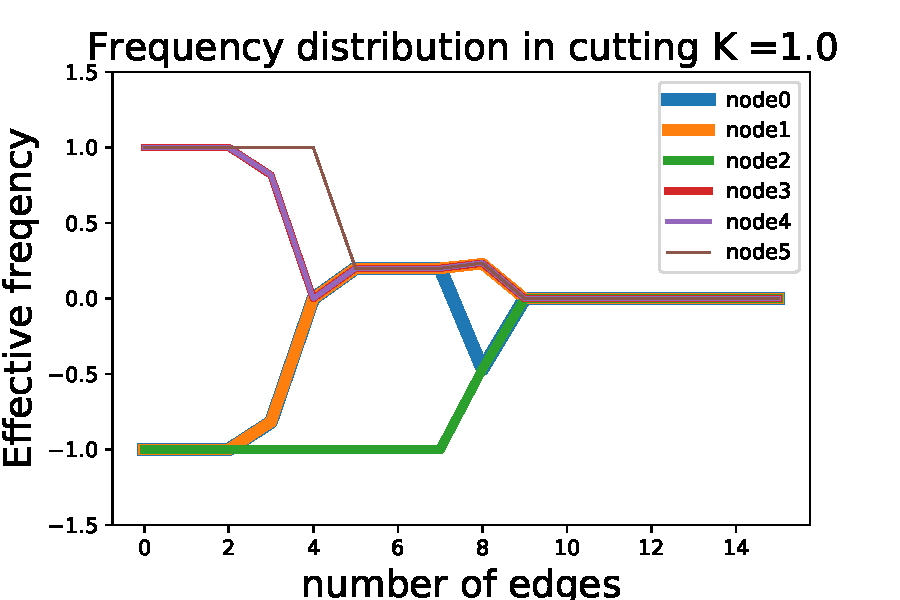
\includegraphics[width=105mm]{./images/cutting_N6K1.pdf}
\centering
\caption{固有振動数$1$の振動子3つと固有振動数の$-1$の振動子3つからなる6体の振動子ネットワークにおいて,枝を1本ずつランダムに選び全接続まで連続的に増やしたときの各振動子の実効振動数の変化を表す.}
\label{fig:cutting_N6K1}
\end{figure}
\section{鞍替え現象のモデル化}
ある1つの振動子が$M$体の集団から$N$体の別の集団に鞍替えを起こすとき,以下のようにモデル化できる.
\begin{screen}
固有振動数$\omega$の振動子が実効振動数$\omega_M$の$M$体の振動子集団$\Omega_M$との間に$m$本の枝で繋がっており,また,実効振動数$\omega_N$の$N$体の振動子集団$\Omega_N$との間に$n$本の枝で繋がっている.
ただし,振動子集団$\Omega_M$と振動子集団$\Omega_N$との間に枝は存在しないとする.(図\ref{fig:switch})\\
枝の本数$m,n$の変化すると,振動子の実効振動数が変化し鞍替えが生じる.
\end{screen}
\begin{figure}[t]
\centering
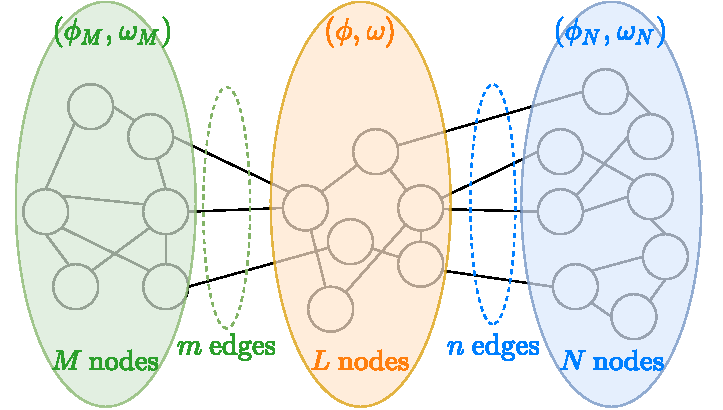
\includegraphics[width=105mm]{./images/three_obj_before.pdf}
\centering
\caption{鞍替え現象に関わる部分ネットワーク}
\label{fig:switch}
\end{figure}
このとき,それぞれの振動子集団に属する振動子について平均化を行うと,発展方程式は以下のようになる.
\begin{align*}
    \dot{\phi}&=\omega+mK\sin\left( \phi_N-\phi \right)+nK\sin\left( \phi_M-\phi \right)\\
    \dot{\phi}_M&=\omega_M+\frac{m}{M}K\sin\left( \phi-\phi_M \right) \\
    \dot{\phi}_N&=\omega_N+\frac{n}{N}K\sin\left( \phi-\phi_N \right)    
\end{align*}
ここで,結合強度比$a=n/m,N=1,M=1$と仮定すると,図\ref{fig:3body}のような鎖状の3体ネットワークに簡略化される.
\begin{figure}[t]
\centering
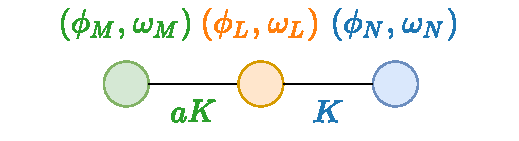
\includegraphics[width=105mm]{./images/three_obj_after.pdf}
\centering
\caption{鞍替え現象に関わる部分ネットワークを簡略化した鎖状の3体ネットワーク}
\label{fig:3body}
\end{figure}
\begin{align}
    \label{eq:3body}
    \begin{split}
        \dot{\phi}&=\omega+K\sin\left( \phi_N-\phi \right)+aK\sin\left( \phi_M-\phi \right)\\
        \dot{\phi}_M&=\omega_M+aK\sin\left( \phi-\phi_M \right) \\
        \dot{\phi}_N&=\omega_N+K\sin\left( \phi-\phi_N \right)    
    \end{split}
\end{align}
\section{3体系の同期状態}
元の部分ネットワーク (図\ref{fig:switch}) における枝の数$m,n$の変化は,3体系 (図\ref{fig:3body}) においてはパラメータ$a,K$の変化に対応する.

3体系について,結合強度比$a$を様々な値で固定し結合強度$K$を変化させたとき,最大で5つの同期状態が存在し,4つの臨界結合強度が存在することがわかった.
特に$a=4.0,\omega=0.1,\Omega=2$は,最も多様に同期状態が変化するパラメータ集合の一つであった.そのときの結合強度と実効振動数の関係を図\ref{fig:3body-state}に示す.
\begin{figure}[t]
\centering
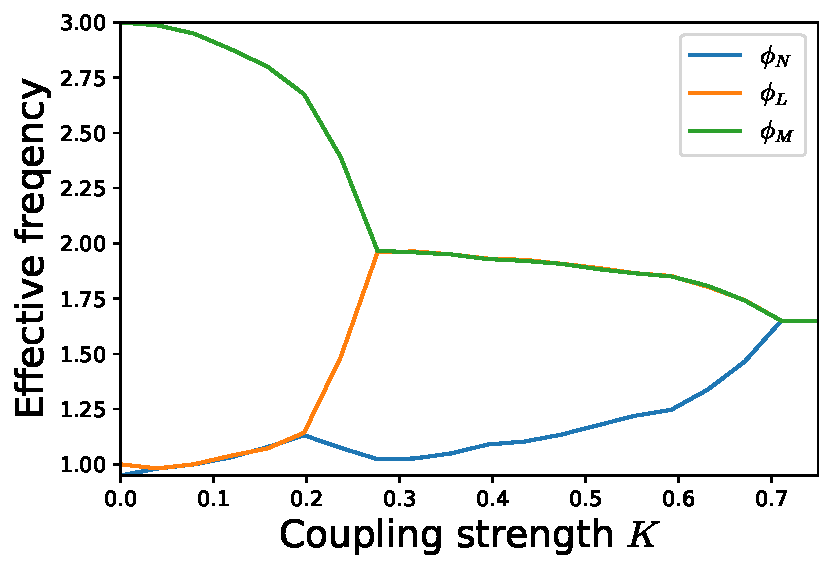
\includegraphics[width=105mm]{./images/three-body-prob.pdf}
\centering
\caption{3体ネットワークで$a=4.0,\omega=0.1,\Omega=2$のしたときの結合強度$K$と実効振動数の関係.$0\leq K\lesssim 0.05$では3体が非同期であり (phase 1),$0.05\lesssim K\lesssim 0.15$では固有振動数の近い2体が同期する($\phi=\phi_N$, phase 2).そして,$0.15 \lesssim K\lesssim 0.27$では鞍替えが起こり非同期になり (phase 3),$0.27\lesssim K\lesssim 0.7$では振動数の遠い2体が同期する ($\phi=\phi_N$,\ phase 4).最後に$K\gtrsim 0.7$では3体が同期する (phase 5).}
\label{fig:3body-state}
\end{figure}
4つの臨界結合強度を分岐点として5つの同期状態に分岐することが分かる.
そこで,4つの臨界結合強度を小さい順にそれぞれ$K_1,K_2,K_3,K_4$とする.
すると,次のようにまとめられる.\\
$0\leq K<K_1$では3体が非同期であり (phase 1),$K_1\leq K<K_2$では固有振動数の近い2体が同期する ($\phi=\phi_N$,\ phase 2).そして,$K_2\leq K<K_3$では鞍替えが起こり非同期になり (phase 3),$K_3\leq K<K_4$では振動数の遠い2体が同期する($\phi=\phi_N$,\ phase 4).最後に$K\leq K_4$では3体が同期する (phase 5).\\
次節ではこれらの5つの同期状態が相平面上でどのように記述されるかを調べる.
\section{3体系の同期状態の相平面解析}
$x=\phi_M-\phi,y=\phi_N-\phi$と位相差を取ると,式\eqref{eq:3body}は2本の位相差方程式になる.
\begin{align}
    \label{eq:phase-diff}
    \begin{split}
    \dot{x}&=\Omega-K(2a\sin x+\sin y)\\
    \dot{y}&=\omega-K(a\sin x+2\sin y)
    \end{split}
\end{align}
また,方程式の対称性から$\Omega\gg\omega$を仮定する.\\
図\eqref{fig:3body-state}のそれぞれの同期状態に対応する$x-y$平面上の相図を図\ref{fig:phase}に示す.

\captionsetup[figure]{justification=centering}
\begin{figure}[t]
    \begin{minipage}[b]{0.47\linewidth}
      \centering
      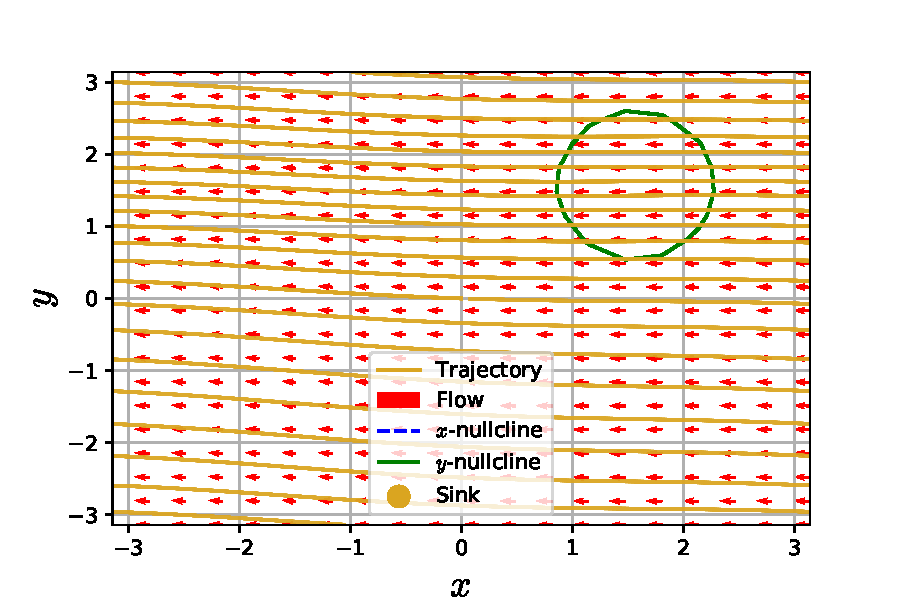
\includegraphics[keepaspectratio, scale=0.42]{images/phase_a4K2.pdf}
      \subcaption{$K=0.02$.3体が非同期.\\phase 1}
      \label{fig:phase-k2}
    \end{minipage}
    \begin{minipage}[b]{0.47\linewidth}
      \centering
      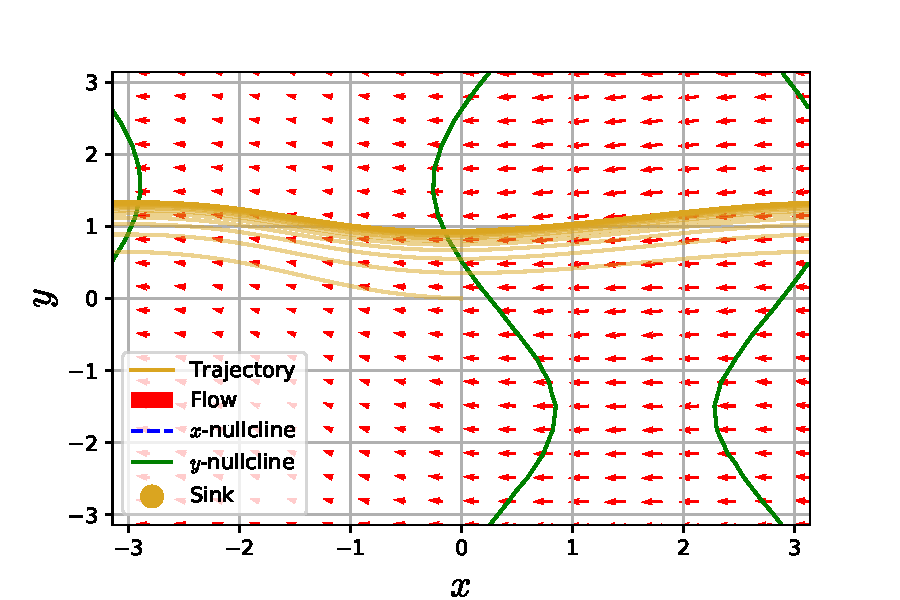
\includegraphics[keepaspectratio, scale=0.42]{images/phase_a4K10.pdf}
      \subcaption[c]{$K=0.1$.固有振動数が近いものと同期.\\phase 2}
      \label{fig:phase-k10}
    \end{minipage}\\
    \begin{minipage}[b]{0.47\linewidth}
      \centering
      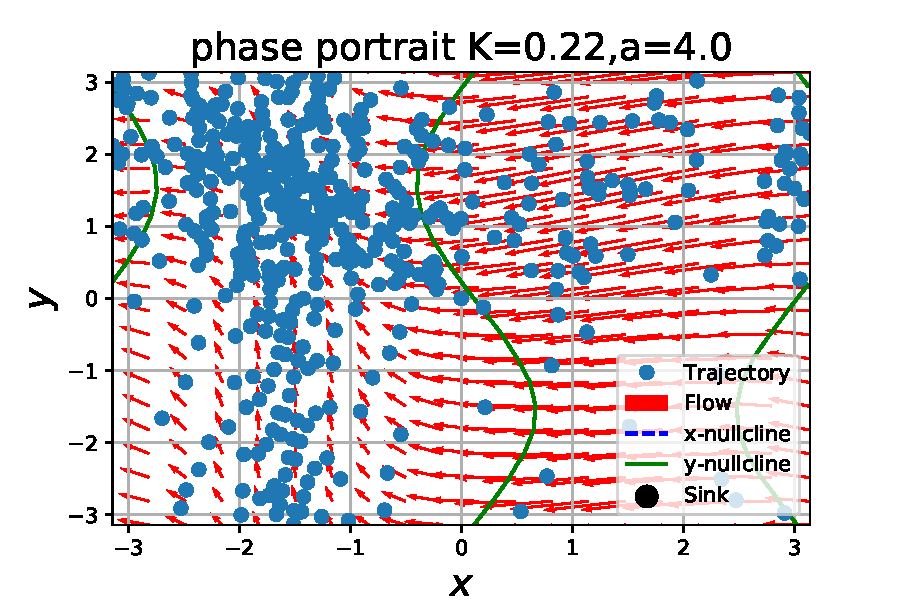
\includegraphics[keepaspectratio, scale=0.42]{images/phase_a4K22.pdf}
      \subcaption{$K=0.22$.鞍替え後3体が非同期.\\phase 3}
      \label{fig:phase-k22}
    \end{minipage}
    \begin{minipage}[b]{0.47\linewidth}
      \centering
      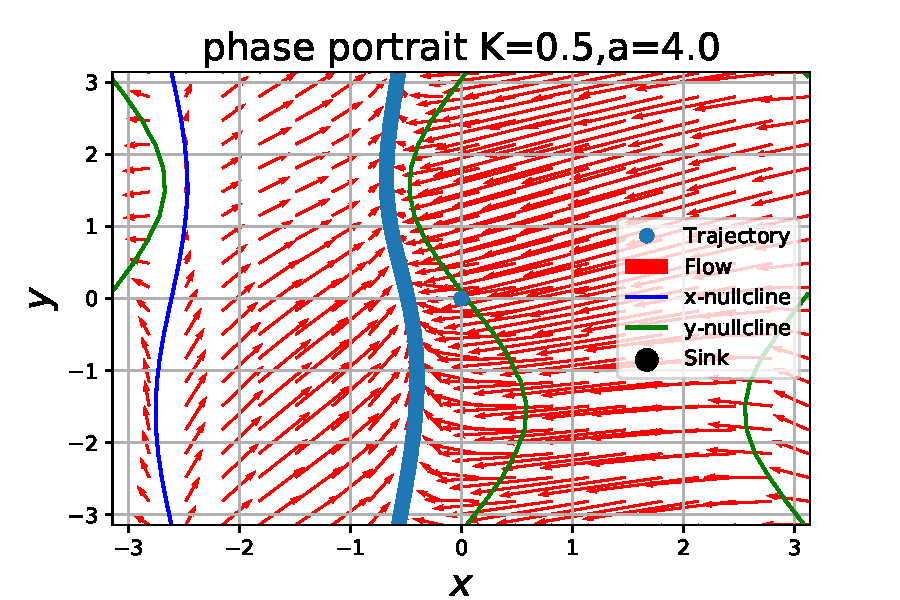
\includegraphics[keepaspectratio, scale=0.42]{images/phase_a4K50.pdf}
      \subcaption{$K=0.5$.固有振動数が遠いものと同期.\\phase 4}
      \label{fig:phase-k50}
    \end{minipage}\\
    \begin{minipage}[b]{0.47\linewidth}
      \centering
      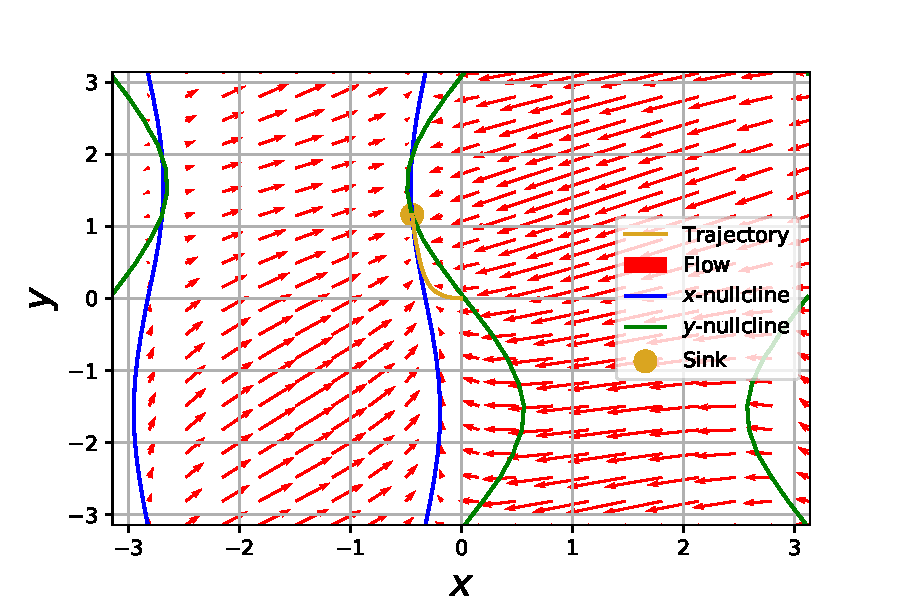
\includegraphics[keepaspectratio, scale=0.42]{images/phase_a4K80.pdf}
      \subcaption{$K=0.8$.3体とも同期.\\phase 5}
      \label{fig:phase-k80}
    \end{minipage}
    \caption{5つの同期状態における相図.$a=4.0,\omega=0.1,\Omega=2$}\label{fig:phase}
\end{figure}
\clearcaptionsetup{figure}

それぞれの同期状態は2本の位相差方程式の安定解に対応し,それぞれ以下のような現象に対応する.
\begin{itemize}
    \item 
    2振動子の同期:任意の初期位相差から位相差$x,y$の片方のみが安定な$\mathbb{S}^1$と同相な周期軌道へ収束する.(図\ref{fig:phase-k10},\ \ref{fig:phase-k50})
    \item
    3振動子の同期:任意の初期位相差から位相差$x,y$の両方とも安定な平衡点へ収束する.(図\ref{fig:phase-k80})
    \item
    非同期:安定な周期軌道が存在せず,準周期軌道を描く.(図\ref{fig:phase-k2},\ \ref{fig:phase-k22})
\end{itemize}
以上の相平面解析の結果を元に,以降の節では4つ臨界結合強度を求める.
\section{臨界結合強度の近似解}
\subsection{固有振動数の近い2体との同期 ($K_1$,$K_2$)}
固有振動数差$\Omega,\omega$に比べ,結合強度$K$が小さい状況($K\leq K_1$)では,以下の大小関係が成り立つ.
\begin{align}
    \label{eq:k1-approx}
    \Omega\gg\omega>K
\end{align}
また,
結合強度$K$が固有振動数差$\Omega$に比べ小さく,固有振動数差$\omega$に比べ大きい状況($K\sim K_2$)では,以下の大小関係が成り立つ.
\begin{align}
    \label{eq:k2-approx}
    \Omega\gg K>\omega
\end{align}
式\eqref{eq:k1-approx},\eqref{eq:k2-approx}両方の状況とも,平均的に$x$は固有振動数$\Omega$で変化し,$y$は$\omega\ll\Omega$で変化する.
よって,タイムスケールの分離を行うことができる.
つまり,$\dot{x}=\Omega, y=z\ (z:\textrm{const})$に対して,$\omega,K$に依存した周期外力が摂動した系として近似できる.\\
    $\tilde{y}:=y/\Omega,\epsilon:=\omega/\Omega,k=K/\Omega,S(x,y)=-a\sin x-2\sin y$とすると,位相差$y$の時間発展は以下のように表される.
    \begin{align*}
        \dv{\tilde{y}}{t}=\epsilon+k S(x,y) 
    \end{align*}
    このとき,$y$が以下のように近恒等変換されると仮定する.
    \begin{align}
        \tilde{y}=z+kh_1(z,t)+k^2h_2(z,t)+O(k^3)
        \label{eq:pertu-ytilde}
    \end{align}
    このとき,$h_i$は$i=1,2,\ h_i(z+2\pi,t+2\pi/\Omega)=h_i(z,t),h(z,0)=0$を満たす関数である.
    一方$x$については$k$の1次で展開すると,
    \begin{align*}
        x&=\Omega t-\Omega k\int_0^t(2a\sin \Omega\tau+\sin\Omega (z+\epsilon\tau)\dd{\tau}+O(k^2)\\ 
        &=\Omega t+\Omega k\left(\frac{2a}{\Omega}\cos\Omega t+t\sin \Omega z\right)+O(k^2)
    \end{align*}
    最終行では,$\cos x(0)=0,\cos y(0)=0$となるように初期時刻$t=0$を定めたことに因る.
    また,$S(x,y)$を$z,t$に関して展開する.
    \begin{align*}
        S(x,y)&=-a\sin x-2\sin y\\
        &=-a\sin\Omega t-2\sin \Omega z-2\Omega kh_1\cos\Omega z\\
        &-a\cos\Omega t\cdot \Omega k\left(\frac{2a}{\Omega}\cos \Omega t+t\sin \Omega z\right)+O(k^2)\\
        &=-a\sin\Omega t-\!2\sin \Omega z       +k\left(\!-2\Omega z \cos\Omega z\cdot h_1-\!2a^2\cos^2\Omega t-\!a\Omega t\cos \Omega  t\sin \Omega z\right)\\
        &+O(k^2)
    \end{align*}
    さらに,$S_1:=-a\sin\Omega t-2\sin\Omega z,S_2:=-2a^2\cos^2\Omega t-a\Omega t\cos \Omega t\sin \Omega z$と定めると,
    \begin{align*}
        S(x,y)=S_1+k\Omega\pt_y S_1\cdot h_1+kS_2
    \end{align*}
    となる.\\
    式\eqref{eq:pertu-ytilde}を両辺$t$で微分すると,
    \begin{align*}
        \dv{\tilde{y}}{t}&=\dot{z}+k(\dot{z}\partial_zh_1+\partial_th_1)+k^2(\dot{z}\partial_zh_2+\partial_th_2)+O(k^3)\\
        &=(1+k\partial_zh_1+k^2\partial_zh_2)\dot{z}+k\pt_th_1+k^2\pt_th_2+O(k^3)
    \end{align*}
    整理すると,
    \begin{align*}
        \dot{z}&=(1+k\pt_zh_1+k^2\pt_zh_2)^{-1}\left( \dv{\tilde{y}}{t}-k\pt_th_1-k^2\pt_th_2 \right)+O(k^3)\\
        &=(1-k\pt_zh_1-k^2\pt_zh_2)\left(\epsilon+kS_1+k^2\Omega \pt_y S_1h_1+k^2S_2-k\pt_th_1-k^2\pt_th_2 \right)\\
        &=\epsilon+k(S_1-\pt_th_1-\epsilon\pt_zh_1)\!+\!k^2\left(\Omega \pt_y S_1h_1 -\pt_th_2-\epsilon\pt_zh_2 -\pt_zh_1(S_1-\pt_th_1)+S_2\right)
    \end{align*}
    $\dot{z}$が以下のように展開されるとする.
    \begin{align*}
        \dot{z}=\epsilon+kH_1(z-\epsilon t)+k^2H_2(z-\epsilon t)+O(k^3)
    \end{align*}
    このとき,$k$の1次を比較すると新たな変数$\tau$を用いて以下の式が成立する.
    \begin{align*}
        H_1(z-\epsilon t)=S_1(z+\epsilon\tau,t+\tau)-\pt_\tau h_1(z+\epsilon\tau,t+\tau)
    \end{align*}
    $\tau=0$から$\tau=-t$で両辺積分すると,
    \begin{align}
        -tH_1(z-\epsilon t)&=\int_0^{-t}\left(-a\sin\Omega(t+\tau)-2\sin\Omega(z+\epsilon\tau)\right)\dd{\tau}+h_1(z,t)\\
        &=\frac{a}{\Omega}\sin\Omega t+\frac{2}{\Omega \epsilon}(\cos \Omega (z-\epsilon t)-\cos \Omega z)+h_1\\
        &=\frac{a}{\Omega}\sin\Omega t+\frac{2}{\Omega \epsilon}(\cos \Omega z+\Omega \epsilon t\sin \Omega z-\Omega^2\epsilon^2t^2/2\cdot\sin \Omega z-\cos \Omega z)+h_1\\
        &=\frac{a}{\Omega}\sin\Omega t+2t\sin \Omega z-\Omega\epsilon t^2\cos \Omega z+h_1+O(\epsilon^2)
        \label{eq-h1-H1}
    \end{align}
    $t=-2\pi/\Omega$を代入して,
    \begin{align*}
        \frac{2\pi}{\Omega}H_1\left(z+\epsilon\frac{2\pi}{\Omega}\right)&=-\frac{4\pi}{\Omega}\sin\Omega z-\frac{4\pi^2}{\Omega}\epsilon \cos \Omega z+O(\epsilon^2)\\
        H_1\left(z+\epsilon\frac{2\pi}{\Omega}\right)&=-2 \sin\Omega z-2\pi\epsilon \cos \Omega z+O(\epsilon^2)\\
        H_1\left(z+\epsilon\frac{2\pi}{\Omega}\right)&=H_1(z)+H_1'(z)\epsilon\frac{2\pi}{\Omega}+O(\epsilon^2)
    \end{align*}
    下2式を比較すると,
    \begin{align*}
        H_1(z)=-2\sin\Omega z+2\pi\epsilon \cos\Omega z+O(\epsilon^2)
    \end{align*}
    が得られる.
    式\eqref{eq-h1-H1}に代入すると,
    \begin{align*}
        h_1(z,t)&=2t\sin\Omega(z-\epsilon t)-2\pi\epsilon t\cos\Omega(z-\epsilon t)-\frac{a}{\Omega}\sin\Omega t-2t\sin \Omega z+\Omega\epsilon t^2\cos \Omega z\\
        &=2t(\sin\Omega z-\Omega \epsilon t\cos\Omega z-\sin\Omega z)-\frac{a}{\Omega}\sin\Omega t+\epsilon(-2\pi t+\Omega t^2)\cos \Omega z+O(\epsilon^2)\\
        &=-\frac{a}{\Omega}\sin\Omega t-\epsilon(2\pi t+\Omega t^2)\cos \Omega z+O(\epsilon^2)
    \end{align*}
    $\dot{z}のk$の2次を比較し,$h_1$を代入する.
    \begin{align*}
        H_2(z-\epsilon t)&=\Omega \pt_y S_1h_1 -\pt_th_2-\epsilon\pt_zh_2 -\pt_zh_1(S_1-\pt_th_1)+S_2\\
        &=-2\Omega \cos \Omega z\left( -\frac{a}{\Omega}\sin\Omega t-\epsilon(2\pi t+\Omega t^2) \cos \Omega z \right)-\pt_\tau h_2\\
        &-2a^2\cos^2\Omega t-a\Omega t\cos \Omega t\sin \Omega z+O(\epsilon^2)\\
        &+\epsilon(2\pi\Omega t+\Omega^2 t^2)\sin\Omega z \left( -a\sin\Omega t-2\sin\Omega z +a\cos\Omega t+\epsilon(2\pi +2\Omega t)\cos\Omega z\right)
    \end{align*}
    両辺$\tau=0$から$\tau=-t$で積分して,$\sin\Omega t\sim 0,\cos\Omega t\sim 1$とすると,
    \begin{align*}
        -tH_2(z-\epsilon t)&=2a\cdot -\epsilon t\sin\Omega z+4\pi\epsilon\Omega\left( -\frac{t^2}{4} -\frac{t^2}{4}\cos 2\Omega z\right)+2\epsilon\Omega^2\left( -\frac{t^3}{6} -\frac{t^3}{6}\cos 2\Omega z\right)\\
        &-2\pi a\epsilon\Omega\cdot\left(\frac{t}{\Omega}\sin\Omega z\right)+2\pi a\epsilon\Omega\left(-\frac{\epsilon t}{\Omega}\cos\Omega z\right)\\
        &-4\pi\epsilon\Omega\left(-\frac{t^2}{4}+\frac{t^2}{4}\cos 2\Omega z\right)-2\epsilon\Omega^2\left( -\frac{t^3}{6} +\frac{t^3}{6}\cos 2\Omega z\right)+O(\epsilon^2)\\
        &-a\epsilon\Omega^2\left( \frac{t^2}{\Omega}\sin\Omega z \right)+a\epsilon\Omega^2\left( -\frac{2t^2}{\Omega}\sin\Omega z \right)\\
        &-2a^2\left( -\frac{t}{2}-\frac{1}{4\Omega} \sin 2\Omega t\right)-a\Omega \left( -\frac{t}{\Omega} \cos\Omega z\right)\\
        &=-2a\epsilon t\sin\Omega z-2\pi\epsilon\Omega t^2\cos 2\Omega z-\frac{2}{3}\epsilon\Omega^2t^3\cos 2\Omega z\\
        &-2\pi a\epsilon t\sin\Omega z-3a\epsilon\Omega t^2\sin\Omega z+at(a+\cos\Omega z)+\frac{a^2}{2\Omega}\sin 2\Omega t
    \end{align*}
    $t=-2\pi/\Omega$を代入して整理すると,
    \begin{align*}
        &H_2(z+\epsilon 2\pi/\Omega)=-a(a+\cos\Omega z)\\
        +&2\epsilon\left( a\sin\Omega z-2\pi^2\cos2\Omega z+\frac{4\pi^2}{3} \cos 2\Omega z+\pi a\sin\Omega z-3\pi a\sin\Omega z\right)
    \end{align*}
    以上で,位相差$y$の近恒等変換$z$の従う微分方程式を近似的に求めることができる.
    よって,$z$が安定解を持つ条件を求めることで$y$が安定解を持つ条件を求めることができる.\\
    まず,式\eqref{eq:k1-approx}の状況では,
    \begin{align*}
        \dot{z}&=\epsilon-2k\sin\Omega z
    \end{align*}
    となる.これは,式\eqref{eq:phase-diff}に対し$x$の周期で平均化を行った($\sin x\sim 0$)式である.\\
    $z$が安定解を持つ条件は,
    \begin{align*}
        k\geq\frac{\epsilon}{2}
    \end{align*}
    となり,臨界結合強度$K_1$は,
    \begin{align*}
        K_1=\frac{\omega}{2}
    \end{align*}
    となる.\\
    次に,式\eqref{eq:k2-approx}の状況を考える.
    閉形式で$K_2$を求めるため$\epsilon \ll 1$を仮定すると,$H_2(z)=-a(a+\cos\Omega z)+O(\epsilon)$より,$k,\epsilon$が十分小さいとき,$2$次以下の微小量を無視すると,$z$は以下のような微分方程式に従う.
    \begin{align*}
        \dot{z}&=\epsilon-2k\sin\Omega z-k^2a(a+\cos \Omega z)\\
        &=\epsilon-a^2k^2-k\sqrt{4+a^2k^2}\sin (\Omega z-\alpha)\quad(\alpha:\mathrm{const})
    \end{align*}
    $z$が安定解を持つ条件は,
    \begin{align*}
        |\epsilon-a^2k^2|&\leq k\sqrt{4+(2\pi\epsilon-ak)^2}\\
        0\leq k&\leq \sqrt{\frac{1}{a^4-a^2}\left(2+a^2\epsilon+\sqrt{(2+2a^2\epsilon)^2-\epsilon^2(a^4-a^2)}\right)}
    \end{align*}
    となり,臨界結合強度$K_2$は,
    \begin{align*}
        K_2=\Omega\cdot\sqrt{\frac{1}{a^4-a^2}\left(2+a^2\epsilon+\sqrt{(2+2a^2\epsilon)^2-\epsilon^2(a^4-a^2)}\right)}
    \end{align*}
    となる.    
    \subsection{固有振動数の遠い2体との同期($K_3$)}
    固有振動数の遠い2体との同期については,命題\ref{prop:suff}により,
    \begin{align*}
        K_3\lessapprox \frac{\Omega}{2a-1}
    \end{align*}
    を得た.
    \begin{proposition}
        \label{prop:suff}
        トーラス$\mathbb{T}^2$上の自律系
        \begin{align}
            \label{eq:prop-2phase}
            \begin{split}
                \dot{x}&=\Omega-K(2a\sin x+\sin y)\\
                \dot{y}&=\omega-K(a\sin x+2\sin y)
            \end{split}
        \end{align}
        において,平衡点を持たず,任意の$y$に対し$\dot{x}=0$が解を持つならば,
        つまり,$K,a$が
        \begin{align*}
            K\geq \frac{\Omega}{2a-1}
        \end{align*}
        を満たすならば,
        2つの安定,不安定な$x$-$\mathrm{nullcline}$付近に$\mathbb{S}^1$と同相な安定,不安定な周期解がそれぞれ存在し,任意の点から発する軌道は2つの周期解のどちらかに収束する.
    \end{proposition}
    まず,以下の補題を示す.
    \begin{lemma}
        \label{lemma:annulus}
        命題\ref{prop:suff}の状況で
        安定な$x$-nullclineの$x$座標の最大値・最小値をそれぞれ$x_{\max},x_{\min}$とし,$D=[x_{\min},x_{\max}]\times (-\pi,\pi ]\subset\mathbb{T}^2$とする.
        このとき,円筒領域$D$内に$\mathbb{S}^1$に同相な安定な周期解がただ一つ存在する.        
    \end{lemma}
    \begin{proof}
        まず,$D$内の任意の点から発する軌道は$D$内に留まる.
        なぜなら,$D$内の点から発して$D$外に出る軌道が存在すると仮定すると$D$の境界上で$D$外の流れを持つが,図\ref{fig:phase-k50}よりそのような点は存在しないからである.\\
        そして,命題\ref{prop:suff}の仮定より平衡点は存在せず,$D$は円環に同相でトーラス$\mathbb{T}^2$と同相でない.\\
        以上より,Poincaré-Bendixsonの定理の一般化 (定理\ref{thm:poiben-gen}) から$D$内に$\mathbb{S}^1$に周期解がただ一つ存在する.
        また,その周期解は安定な$x$-nullclineと交差することから安定な周期解である.        
    \end{proof}
    次に命題\ref{prop:suff}の証明を示す.
    \begin{proof}
        補題\ref{lemma:annulus}と式\eqref{eq:prop-2phase}の座標・時刻に対する対称性から,安定な$x$-nullclineと不安定な$x$-nullclineの付近にそれぞれ安定,不安定な周期解$\gamma_a,\gamma_b$を持つ.\\
        他に周期解$\gamma$が存在すると仮定すると,$\gamma$は$\gamma_a,\gamma_b$と交わることはないので,任意の$y\in(-\pi,\pi]$に対し,ある$x\in(-\pi,\pi]$が存在して,$(x,y)\in\gamma$となる.
        また,そのような周期解は$x$-nullclineと交わる必要がある.なぜなら,$x$-nullclineと交わるまで流れの$x$成分の符号が変わらないので必ず$x$-nullclineの吸収領域に到達するからである.
        しかし,補題\ref{lemma:annulus}より,1つの$x$-nullclineは1つの周期解としか交わらないため矛盾する.
        最後に,Poincaré-Bendixsonの定理の一般化 (定理\ref{thm:poiben-gen}) により,任意の点から発する軌道は$\gamma_a,\gamma_b$のいずれかに収束する.
    \end{proof}
\subsection{3体の同期($K_4$)}
式\eqref{eq:phase-diff}が平衡点を持つとき,
平衡点は,
\begin{align*}
    (x,y)=\left(\arcsin \frac{2\Omega-\omega}{3aK},\arcsin \frac{2\omega-\Omega}{3K}\right)
\end{align*}
となる.
よって,平衡点の存在条件は,
\begin{align*}
    K\geq \frac{2\Omega-\omega}{3a}\ \cap \ K\geq \frac{\Omega-2\omega}{3}
\end{align*}
となる.
さらに,平衡点が存在するとき,平衡点は源点・沈点・2つの鞍点である (図\ref{fig:phase-k80}).
このとき,源点から2つの鞍点へ,2つの鞍点から沈点への流れがあるので,鞍点の安定多様体と交わるようなLimit Cycleは存在しない.
また,全ての平衡点は$x,y$-nullclineの交点であるので,源点を囲うようなLimit Cycleも存在しない.
よって,平衡点を持つとき,周期解は持たず,Poincaré-Bendixsonの定理の一般化 (定理\ref{thm:poiben-gen}) から任意の点から発する軌道は沈点へ収束する.
以上より,3体が同期する臨界結合強度$K_4$は,
\begin{align*}
    K_4=\max\left(\frac{2\Omega-\omega}{3a},\frac{\Omega-2\omega}{3}\right)
\end{align*}
となる.

\end{document}